\newcommand{\KiekerTerminology}[1]{{\small\sffamily #1}}
\newcommand{\MonitoringProbe}{\KiekerTerminology{Monitoring Probe}}
\newcommand{\MonitoringProbes}{\KiekerTerminology{Monitoring Probes}}
\newcommand{\MonitoringLog}{\KiekerTerminology{Monitoring Log}}
\newcommand{\MonitoringLogWriter}{\KiekerTerminology{Monitoring Log Writer}}
\newcommand{\MonitoringLogWriters}{\KiekerTerminology{Monitoring Log Writers}}
\newcommand{\MonitoringLogReader}{\KiekerTerminology{Monitoring Log Reader}}
\newcommand{\MonitoringLogReaders}{\KiekerTerminology{Monitoring Log Readers}}
\newcommand{\MonitoringRecord}{\KiekerTerminology{Monitoring Record}}
\newcommand{\MonitoringRecords}{\KiekerTerminology{Monitoring Records}}
\newcommand{\MonitoringRecordConsumer}{\KiekerTerminology{Monitoring Record Consumer}}
\newcommand{\MonitoringRecordConsumers}{\KiekerTerminology{Monitoring Record Consumers}}
\newcommand{\KiekerTpmon}{\KiekerTerminology{Kieker.Tpmon}}
\newcommand{\KiekerTpan}{\KiekerTerminology{Kieker.Tpan}}
\newcommand{\TpmonController}{\KiekerTerminology{TpmonController}}
\newcommand{\TpanInstance}{\KiekerTerminology{TpanInstance}}

\noindent This section provides an overview of Kieker's framework
architecture.
The outstanding features of Kieker may be summarized as follows:
 \begin{itemize}
 \item A common, extensible monitoring record model that is shared among the logging and analysis component: in this paper, we use record types for storing response times (in this section), %
 and (distributed) trace information~(Sections~\ref{sec:tracing} and~\ref{sec:casestudy}). % we could also record resource utilization data or other system information that is measurable.
 \item An extensible reader/writer model: the monitoring records may be written to and being read from relational databases, to the file~system or to JMS queues; additional data sinks may be added.
\pagebreak
 \item An extensible monitoring record consumer model: the monitoring records may be analyzed and visualized for various purposes.  If the monitoring log is based on a messaging middleware, continuous online analysis is supported.
 \end{itemize}
 
\noindent The Unified Modeling Language~(UML)~%
\citep{OMG2007UML22Superstructure} is employed for describing the architecture, independent of the programming language (which is Java for Kieker).

\begin{figure}\centering
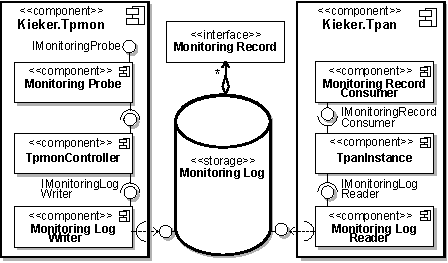
\includegraphics[width=1\columnwidth]{figures/kiekerComponentDiagram-woCloud-bw}%
\caption{Top-level view on Kieker's architecture}
\label{fig:kieker:coreFrameworkComponents}
\end{figure}

At the top-level, Kieker is partitioned into the two components \KiekerTpmon{} and %
\KiekerTpan{} with the \MonitoringLog{} in between, as illustrated in Figure~\ref{fig:kieker:coreFrameworkComponents}. %
\KiekerTpmon{} provides a reusable infrastructure for collecting %
application-level monitoring data in \MonitoringProbes{} and writing this %
monitoring data to the \MonitoringLog{}, e.g., the local file system, a database, or %
a messaging queue, using a \MonitoringLogWriter{}. %
The \TpmonController{} %
is responsible for initializing and controlling a \KiekerTpmon{} instance. %
The \MonitoringLog{} contains \MonitoringRecords{}, as defined in Figure~%
\ref{fig:kieker:coreFrameworkComponents}. %TR: \ref{fig:kieker:coreFrameworkClassesAndInterfaces:record}. 
Each record holds the %
monitoring data of a single measurement created by the \MonitoringProbes{}. %
\KiekerTpan{} provides the infrastructure for analyzing the \MonitoringLog{}: %
a \MonitoringLogReader{}~(Figure~\ref{fig:kieker:coreFrameworkComponents}) reads \MonitoringRecords{} from the %
\MonitoringLog{} and delivers these to registered \MonitoringRecordConsumers{}, according to the observer design pattern~\citep{GammaHelmJohnsonVlissides1995DesignPatternsElementsOfReusableObjectOrientedSoftware}. %
\MonitoringRecordConsumers{} perform the actual analysis or visualization functionality. %
A \KiekerTpan{} instance is initialized and controlled by a \TpanInstance{} %
instance (Figure~\ref{fig:kieker:coreFrameworkComponents}). %

\begin{figure}
\centering
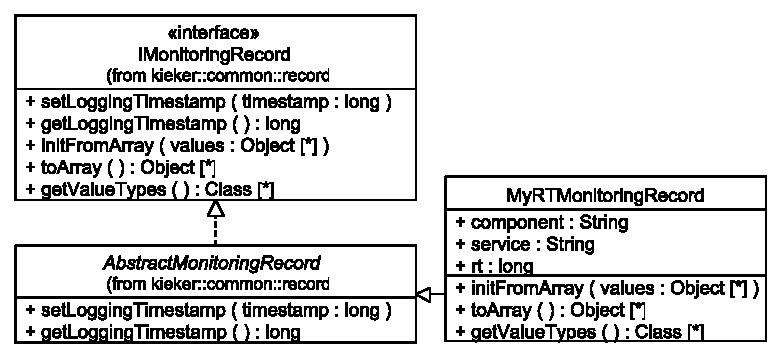
\includegraphics[scale=0.65]{figures/model/kieker_MyRTMonitoringRecord}%
% TR: \includegraphics[width=0.9\columnwidth]{figures/KiekerInterfaceOverviewReArranged-woMonitoringRecord-bw-record-withRTRecord}%
\caption{Monitoring Record interface and abstract class, as well as a concrete Monitoring Record as example.}
\label{fig:kieker:coreFrameworkClassesAndInterfaces:record}
\end{figure}

\begin{figure}\centering
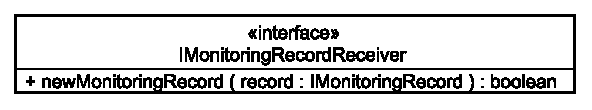
\includegraphics[scale=0.65]{figures/model/kieker_IMonitoringRecordReceiver}
\caption{Monitoring Record Receiver}
\label{fig:record:IMonitoringRecordReceiver}
\end{figure}

\begin{figure}\centering
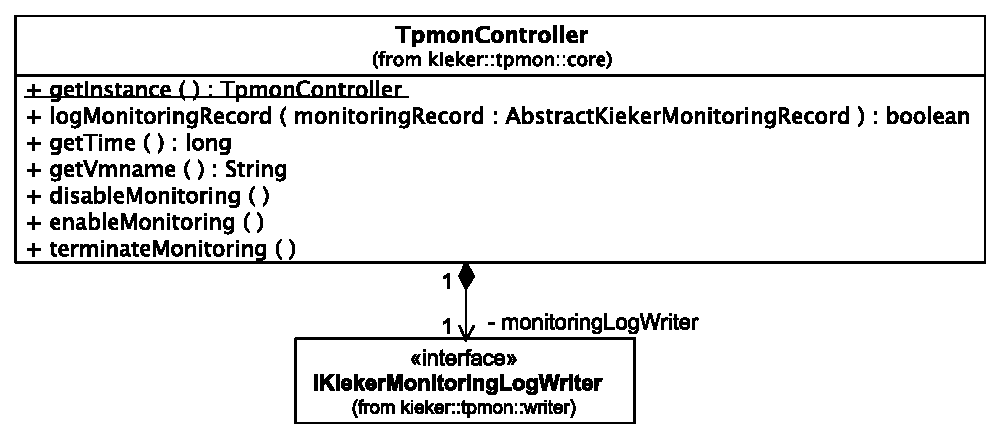
\includegraphics[scale=0.65]{figures/model/kieker_TpmonController}% 
% TR: \includegraphics[scale=0.69]{figures/KiekerInterfaceOverviewReArranged-woMonitoringRecord-bw-tpmon}%
\caption{Kieker.Tpmon}
\label{fig:kieker:coreFrameworkClassesAndInterfaces:tpmon}
\end{figure}

\begin{figure}\centering
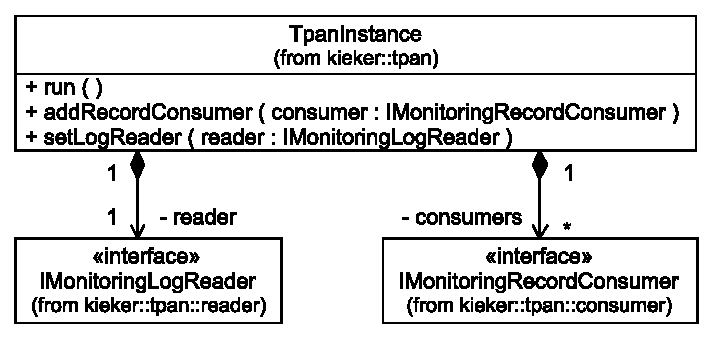
\includegraphics[scale=0.65]{figures/model/kieker_TpanInstance}%
% TR: \includegraphics[scale=0.69]{figures/KiekerInterfaceOverviewReArranged-woMonitoringRecord-bw-tpan}%
\caption{Kieker.Tpan}
\label{fig:kieker:coreFrameworkClassesAndInterfaces:tpan}
\end{figure}

\begin{figure*}\centering
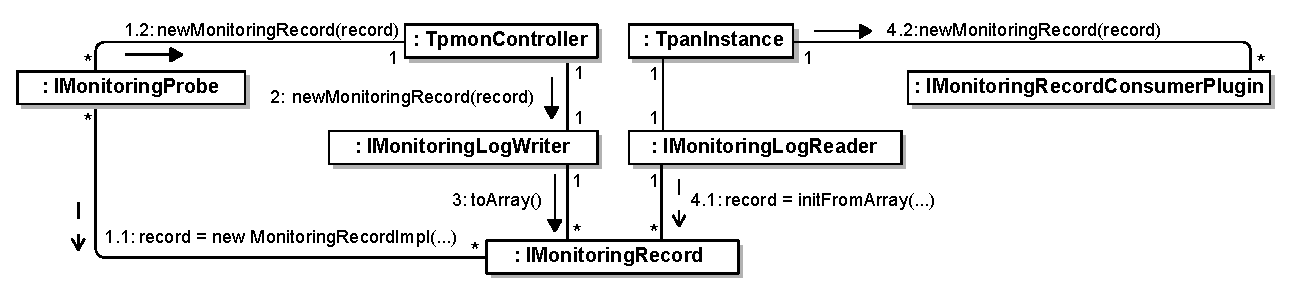
\includegraphics[width=0.8\textwidth]{figures/kiekerCommunications-revisedReArranged-woMonitoringLog-bw}%
\caption{Communication among framework components %
%{\textcolor{red}{S\"{o}ren: Evtl. spezifischer angeben, welche Kommunikation gezeigt wird? Im Text ist vom Life-Cycle eines Monitoring-Records die Rede}}
for creating and writing a Monitoring Record in Kieker.Tpmon~(1.1--3) as well as %
reading and using this Monitoring~Record in Kieker.Tpan~(4.1,~4.2). %
}
\label{fig:kieker:communicationsAmongCoreFrameworkComponents}
\end{figure*}

Figure~\ref{fig:kieker:coreFrameworkClassesAndInterfaces} shows the core
% \WH{etwas Erl\"{a}uterung zu den Assoziationen?}
% Anm. Andr\'{e}: Ja, hier koennte man noch mehr erklaeren ...
Kieker framework classes and interfaces with their associations in a UML~Class %
Diagram notation. %
Kieker offers different implementations for the \MonitoringRecord{}, %
\MonitoringProbe{}, \MonitoringLogWriter{}, %
\MonitoringLogReader{}, and \MonitoringRecordConsumer{} %
components and allows to use customized components created by implementing or %
extending the interfaces or abstract classes of the framework corresponding to these components, as described below.
% 
% % \newpage
% 
Figure~\ref{fig:kieker:communicationsAmongCoreFrameworkComponents} illustrates a \MonitoringRecord{}'s life cycle. It shows the
sequence of interactions among instances of the
Kieker components in a UML~Communication Diagram
notation, whereby the numbers at the operation calls, which are attached to the links, define the order. The multiplicities at the links indicate the possible number of these links among respective object instances.


% \subsection{Framework Components}

% A singleton~%
% \cite{GammaHelmJohnsonVlissides1995DesignPatternsElementsOfReusableObjectOrientedSoftware} %
% instance of t

% \newpage

\subsection{Monitoring Record}\label{sec:architecture:record}

\noindent A \MonitoringRecord{} holds the measurement data collected in a single measurement. %
Different types of \MonitoringRecords{} can be used together in one \KiekerTpmon{} %
instance. %
Figure~\ref{fig:kieker:coreFrameworkClassesAndInterfaces:record} shows a %
concrete \MonitoringRecord{} type \classname{MyRTMonitoringRecord} which can be used %
to store response times of services provided by software components. %
As required by all \MonitoringRecord{} types, it implements the interface \classname{IMonitoringRecord}---%
in this case by extending the abstract framework class \classname{Abstract\+MonitoringRecord}. %

\subsection{Monitoring Probe}\label{sec:monitoringProbe}
% 
% % \begin{figure}
% % % \begin{minipage}[t]{0.4\textwidth}
% %  \begin{multicols}{2}
% % \parbox{0.45\textwidth}{
% % \subfigure[Probe package]{\label{fig:probePackage}%
% % \includegraphics[width=0.4\textwidth]{figures/monitoringProbe}%
% % }\\\quad\\
% % }\newpage
% % % \end{minipage}
% %
% % \subfigure[Example AspectJ response time probe]{%
% % \includegraphics[width=0.46\textwidth]{figures/probe-example}%
% % }
% % \end{multicols}
% % \caption{TODO}
% % \end{figure}
% 
\noindent A \MonitoringProbe{} (Figure~\ref{fig:kieker:coreFrameworkComponents}) contains the measurement logic which collects and possibly %
pre-processes measurement data from the application. %
A \MonitoringProbe{} creates an instance of a \MonitoringRecord{} and sends this %
\MonitoringRecord{} to the \TpmonController{} by calling the
method \opname{newMonitoringRecord(..)} of the \TpmonController{}, as shown in %
Figure~\ref{fig:kieker:communicationsAmongCoreFrameworkComponents}. %Abstract\+Kieker\+MonitoringRecord record)}. %
All \MonitoringProbe{} types must implement the interface \classname{IMonitoring\+Probe} (Figure~\ref{fig:kieker:coreFrameworkClassesAndInterfaces}). %

\MonitoringProbes{} of different types can be used together in a single \KiekerTpmon{} %
instance and are typically tightly bound to middleware underlying the application. %
% The location of a monitoring probe within an instrumented system is called a %
% \textit{monitoring point}.
For example, the interception APIs of Java middleware technologies provided by the
Spring framework, the Java Servlet specification, and the Apache~CXF Web service
framework can be used to implement and integrate \MonitoringProbes{} into an application. %
In Section~\ref{sec:casestudy}, we demonstrate how different technology-specific
types of \MonitoringProbes{} can be used in combination to monitor distributed traces.

% \begin{minipage}{\columnwidth}
\begin{lstlisting}[float, language=Java, caption=Example AspectJ response time Monitoring Probe, label=lst:aspectJRTMonitoringProbe]
@Aspect
public class MyRTMonitoringProbe
       implements IMonitoringProbe {

 static final TpmonController CTRL =
        TpmonController.getInstance();

 @Around
    (value="execution(@MyRTProbe * *.*(..))")
 public Object probe(ProceedingJoinPoint j)
        throws Throwable {
  MyRTMonitoringRecord record =
                new MyRTMonitoringRecord();
  record.component = j.getSignature()
                      .getDeclaringTypeName();
  record.service = j.getSignature().getName();
  Object retval;
  long tin = CTRL.getTime();
  try { retval = j.proceed(); }
  catch (Exception e) { throw e; }
  finally {
   record.rt = CTRL.getTime() - tin;
   CTRL.newMonitoringRecord(record);
  }
  return retval;
 }
}
\end{lstlisting}
% \end{minipage}

As an example, Listing~\ref{lst:aspectJRTMonitoringProbe} shows an AspectJ-based \MonitoringProbe{} %
which measures response times of Java methods and stores this data as \MonitoringRecords{} %
of the previously introduced type \classname{MyRTMonitoringRecord} (Figure~\ref{fig:kieker:coreFrameworkClassesAndInterfaces:record}). %
In this example, all Java methods annotated with \classname{MyRTProbe} %
are instrumented, as follows for the method \classname{searchBook()} via Java annotation:\\

\begin{minipage}{\columnwidth}
{\small
\begin{verbatim}
@MyRTProbe()
public static void searchBook() { .. }
\end{verbatim}
}
\end{minipage}\\

% Integration into application code:
% \begin{itemize}
% \item Java annotations/AOP (AspectJ)
% \item Interception APIs (Spring, Servlet, CXF)
% \item Manual integration (facade pattern)
% \end{itemize}

% \WH{Gewisse Erl\"{a}uterung zu Listing~\ref{lst:aspectJRTMonitoringProbe} n\"{o}tig}

\noindent Calls to an instrumented method are intercepted and the execution %
proceeds with the method \classname{probe(..)}~(lines~10--26) containing the %
response time measurement logic of the \MonitoringProbe{}. %
Before the execution is delegated to the intercepted method~(line~19), %
a \MonitoringRecord{} instance is created and initialized~(lines~13--16) %
and the timestamp before the execution is taken~(line~18). %
After this execution returns, the response time is calculated and stored in %
the \MonitoringRecord{}~(line~22) which is then passed to the \TpmonController{} %
instance~(line~23).

\subsection{Monitoring Log Writer}\label{sec:monitoringlogwriter}

\begin{figure}\centering
\subfigure[Implemented writers]{\label{fig:writers}%
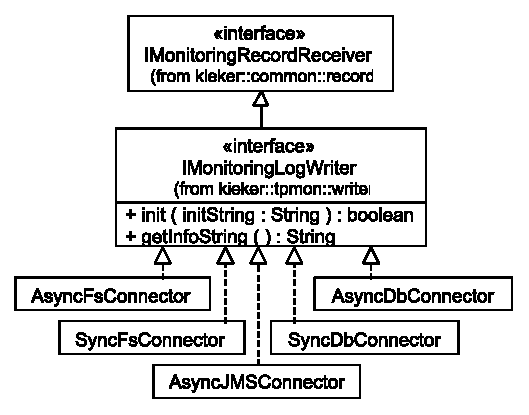
\includegraphics[scale=0.65]{figures/model/kieker_writerimpls}%
% TR: \includegraphics[scale=0.8]{figures/tpmon-writers-refined-bw}%
}\qquad
\subfigure[Implemented readers]{\label{fig:readers}%
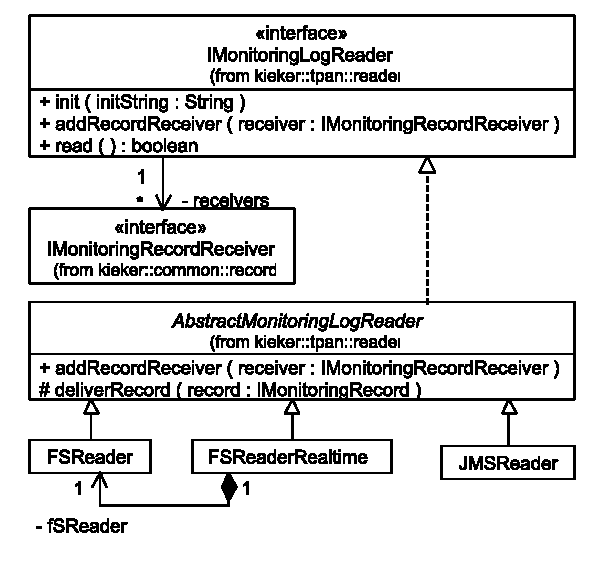
\includegraphics[scale=0.65]{figures/model/kieker_readerimpls}%
%TR: \includegraphics[scale=0.8]{figures/tpmon-readers-refined-bw}%
}
\caption{Implemented monitoring log writers and readers. %The abstract classes have been introduced in Figure~\ref{fig:kieker:coreFrameworkClassesAndInterfaces}.
}
\label{fig:writersAndReader}
\end{figure}

\noindent A \MonitoringLogWriter{} is responsible for writing/serializing the %
\MonitoringRecords{} to the \MonitoringLog{}. %
For each \MonitoringRecord{} to be logged, the writer is invoked
by the \TpmonController{} and writes the data contained in the retrieved \MonitoringRecord{} %
by calling the \MonitoringRecord{}'s \classname{toArray()} method, %
as illustrated in Figure~\ref{fig:kieker:communicationsAmongCoreFrameworkComponents}. %
% A \classname{TpmonController} initializes and uses exactly one monitoring log writer.
Figure~\ref{fig:writers} shows the \MonitoringLogWriters{} which are already included %
in the Kieker framework, supporting the file system, relational databases, and JMS %message
queues. %
The prefixes \textit{Sync/Async} in Figure~\ref{fig:writers} indicate whether the I/O operation required to %
log the \MonitoringRecord{} is performed within the \MonitoringProbe{}'s thread of control~%
(synchronously) or by one or more asynchronous writer thread(s) using an internal buffer. %
The filesystem writer stores \MonitoringRecords{} represented as comma-separated values~(CSV). %
Listing~\ref{lst:RTMonitoringLog} shows a sample filesystem \MonitoringLog{} %
containing entries of the \classname{MyRTMonitoringRecord} \MonitoringRecord{} type. %
Each line contains the \MonitoringRecord{} type identifier, as well as the values
of the record fields \textit{loggingTimestamp}~(cropped in the listing), \textit{component}, \textit{service}, %
and \textit{rt}~(response time in nanoseconds). %
A mapping file is used to store the mapping between a \MonitoringRecord{} type %
identifier and its implementing class, as shown in Listing~\ref{lst:RTMonitoringLogMapping}. %
% %The mapping is required since \MonitoringRecords{} of different type are written to
% %the same file and to allow ...
% 
% % Monitoring log writers must extend the abstract class %
% % \classname{Abstract\+Kieker\+Monitoring\+Log\+Writer}. %
% 
% % \WH{Beispiel kurz erl\"{a}utern? Gut w\"{a}re es evtl ein zweites Record zu haben, damit Listing 4 mehr Sinn macht.}
% % Anm. Andr\'{e}: Ja, w\"{a}re gut ein zweites zu haben; z.B. das in Kieker enthaltene
% %             BranchingRecord, das man verwenden kann, um zu loggen, welche
% %             Ast einer Verzweigung genommen wird.
% %             Aus Zeitgr\"unden habe ich das jetzt nicht mehr gemacht.
\begin{minipage}{\columnwidth}
\begin{lstlisting}[language=Java, numbers=none, xleftmargin=0pt, caption=Filesystem Monitoring Log with Monitoring Records of type MyRTMonitoringRecord, label=lst:RTMonitoringLog, basicstyle=\ttfamily\footnotesize]
$\$$1;..267737726;Catalog;getBook;2104283
$\$$1;..268321753;Catalog;getBook;2679347
$\$$1;..324713919;Catalog;getBook;20082302
$\$$1;..324780416;CRM;getOffers;20164491
$\$$1;..324787610;Bookstore;searchBook;93795571
$\$$1;..325166071;Catalog;getBook;20568496
$\$$1;..325180972;CRM;getOffers;20612072
$\$$1;..325186824;Bookstore;searchBook;94195055
\end{lstlisting}

\begin{lstlisting}[language=Java, numbers=none, xleftmargin=0pt, caption=Mapping of Monitoring Record type identifier to implementing class, label=lst:RTMonitoringLogMapping, basicstyle=\ttfamily\small]
$\$$1=MyRTMonitoringRecord
\end{lstlisting}
\end{minipage}

\subsection{Monitoring Log Reader}

\noindent A \MonitoringLogReader{} is used to create \MonitoringRecord{} instances from %
a \MonitoringLog{} written by a corresponding \MonitoringLogWriter{} (by
calling a \MonitoringRecord{}'s \classname{init\+FromArray(..)} method), see Figure~\ref{fig:kieker:coreFrameworkClassesAndInterfaces:record}. %%
As shown in Figure~\ref{fig:readers}, %
% Monitoring log readers must extend the abstract class %
% \classname{Abstract\+Kieker\+Monitoring\+Log\+Reader}. %
Kieker includes \MonitoringLogReaders{} corresponding to the included writers %
for the filesystem and for JMS queues. %
% \WH{and databases ?}
% Anm. Andr\'{e}: Nein, einen DB-reader haben wir in dieser Implementierung zur Zeit noch nicht.  %
% A \classname{TpanInstance} instance uses exactly one monitoring log reader. %
\MonitoringLogReaders{} extend the abstract class \classname{Abstract\+Monitoring\+Log\+Reader}, %\classname{Abstract\+Kieker\+Monitoring\+Log\+Reader},
which already provides convenient functionality for handling the subscription of %
\MonitoringRecordConsumers{} to \MonitoringRecords{} of specific types as well as %
the delivery of records to the subscribers. %

% Monitoring log readers are also used to replay monitoring logs, e.g., in order
% to run analysis routines with . %
Additionally, Kieker includes the \MonitoringLogReader{} \classname{FSReaderRealtime} %
which can be used to replay \MonitoringRecords{} from a filesystem-based %
\MonitoringLog{} in the original timescale. This has proven to be very helpful for debugging purposes and for simulating %
continuously incoming monitoring data while developing online analysis components. %
% %
% 
\subsection{Monitoring Record Consumer}
% 
% \begin{figure}\centering
% % \subfigure[Kieker.Tpan class diagram]{%
% % \includegraphics[width=0.75\textwidth]{figures/LogAnalysisMetaModel}%
% % }
% % \subfigure[UML Communication Diagram]{%
% 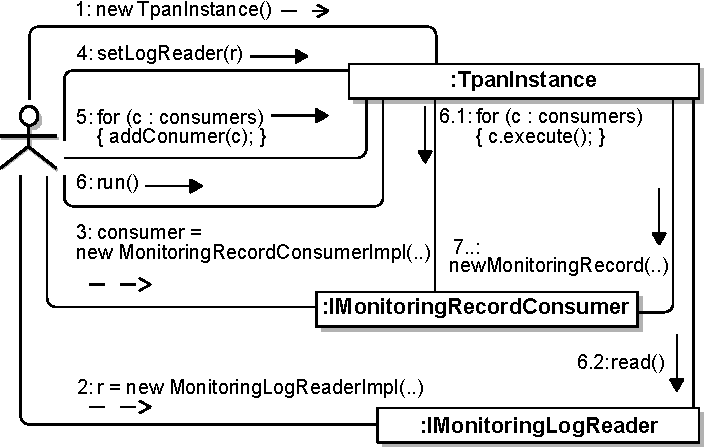
\includegraphics[width=\columnwidth]{figures/LogAnalysisCommunications-bw}%
% % }
% % \subfigure[Code example]{%
% % \includegraphics[width=0.35\textwidth]{figures/logAnalysis-ctrlExample}
% % }
% \caption{Kieker.Tpan communication diagram}
% \label{fig:tpanCommunicationDiagram}
% \end{figure}
% 
\noindent Analysis or visualization components are integrated into \KiekerTpan{} %
by implementing the \classname{IMonitoringRecordConsumer} interface (see Figure~\ref{fig:kieker:coreFrameworkClassesAndInterfaces}). %
A \MonitoringRecordConsumer{} is registered to the \TpanInstance{} as a subscriber
for \MonitoringRecords{} of selected or all \MonitoringRecord{} types %
(as returned by the \classname{getRecordTypeSubscriptionList()} method, see Figure~\ref{fig:kieker:coreFrameworkClassesAndInterfaces}). %
The \TpanInstance{} delegates the subscription list to the \MonitoringLogReader{},
which directly delivers newly incoming records of interest to the consumers by calling their
\classname{consumeMonitoringRecord(..)} method, as illustrated in %
Figure~\ref{fig:tpanCommunicationDiagram}. %

Listing~\ref{lst:rtMonitor} shows an example response time monitor for %
\classname{MyRTMonitoringRecord} that we use as an  example in the present section. %
The monitor compares~(line~19) incoming response time values  with a threshold value %
stored in the object's variable \classname{rtSlo}~(response time service level objective), %
which is specified on object creation~(line~6). %
By returning the classname of the \MonitoringRecord{} type \classname{MyRTMonitoringRecord} %
in line~10, the monitor only receives \MonitoringRecords{} of this type. %
Please remind that Kieker allows to use
the same data structures~(\MonitoringRecords{}) in analysis components as used in the %
\MonitoringProbes{}, in this case the \MonitoringProbe{} measuring the response times %
(Listing~\ref{lst:aspectJRTMonitoringProbe}) and the \MonitoringRecordConsumer{} %
(Listing~\ref{lst:rtMonitor}) implementing the response time monitor.


\begin{lstlisting}[float,language=Java, caption=Example response time monitor, label=lst:rtMonitor,escapechar=\%]
public class RTMonitor
  implements IMonitoringRecordConsumerPlugin {

 private static final 
  Collection<Class<? extends IMonitoringRecord>> 
  recordTypeSubscriptionList =
  new ArrayList<Class<? extends IMonitoringRecord>>();
  static {
   recordTypeSubscriptionList
   .add(MyRTMonitoringRecord.class);
  }

 private final long rtSlo;

 public RTMonitor(long rtSlo) {
  this.rtSlo = rtSlo;
 }

 public 
 Collection<Class<? extends IMonitoringRecord>>
 getRecordTypeSubscriptionList()
 {
   return recordTypeSubscriptionList;
 }

 public 
 void 
 newMonitoringRecord (IMonitoringRecord r) 
 {
  MyRTMonitoringRecord rtRec =
                      (MyRTMonitoringRecord) r;
  if (rtRec.rt > this.rtSlo) {
    /* SLO violation! */
  }
 }

 public boolean execute() { return true; }
 public void terminate() { }
}
\end{lstlisting}

When a \TpanInstance{} is started by calling its \classname{run()} method, the
\classname{execute()} methods of all registered \MonitoringRecordConsumers{} %
are called. %
This allows the implementation of an asynchronous event-based architecture,
which is particularly useful for online analysis components. %
Such an online analysis component spawns a thread in its \classname{execute()} %
method implementing the analysis tasks based on asyncronously incoming \MonitoringRecords{}. %
